\begin{enumerate}

    \item-
    \\
    \textbf{Solución item B:}
    \begin{verbatim}
  (xi,xj)   media_mues     var_mues    P(x1,x2)
    1,1    (1+1)/2 =  1      0.00        0.25
    1,2    (1+2)/2 = 1.5     0.50        0.2
    1,3    (1+3)/2 =  2      2.00        0.05
    2,1    (2+1)/2 = 1.5     0.50        0.2
    2,2    (2+2)/2 =  2      0.00        0.16
    2,3    (2+3)/2 = 2.5     0.50        0.04
    3,1    (3+1)/2 =  2      2.00        0.05
    3,2    (3+2)/2 = 2.5     0.50        0.04
    3,3    (3+3)/2 =  3      0.00        0.01
    
      media_mues     P(X=x)
          1           0.25
         1.5          0.4
          2           0.26
         2.5          0.08
          3           0.01
    \end{verbatim}
    
    \begin{lstlisting}[frame=single]
    x <- c(1, 1.5, 2, 2.5, 3)
    p <- c(0.25, 0.4, 0.26, 0.08, 0.01)
    df2 <- data.frame(x, p)
    library(tidyverse)
    ggplot(df2, aes(x, p))+geom_bar(stat="identity",width=0.25)
    \end{lstlisting}
    
    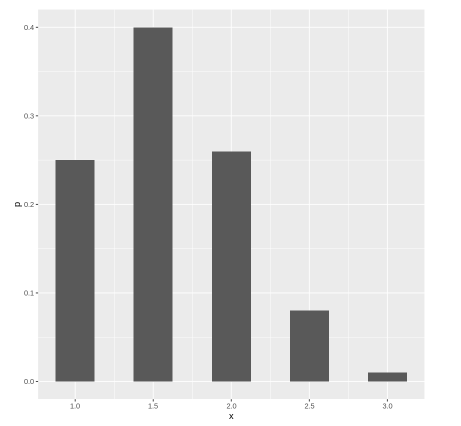
\includegraphics[scale=0.8]{img/m_muest.png}

\end{enumerate}